% !TEX TS-program = xelatex
\documentclass[11pt,a4paper]{ctexart}

% ── Layout ──
\usepackage[margin=2.3cm]{geometry}
\usepackage{setspace}
\onehalfspacing

% ── Graphics & Tables ──
\usepackage{graphicx}
\usepackage{booktabs}
\usepackage{xcolor}
\usepackage{tikz}
\usetikzlibrary{arrows.meta, positioning, shapes.geometric, calc, fit, backgrounds}

% ── Code Listings ──
\usepackage{listings}
\lstset{
  basicstyle=\small\ttfamily,
  breaklines=true,
  frame=single,
  framesep=4pt,
  rulecolor=\color{gray!40},
  backgroundcolor=\color{gray!5},
  showstringspaces=false,
  aboveskip=8pt,
  belowskip=8pt,
}

% ── Headers & Footers ──
\usepackage{fancyhdr}
\pagestyle{fancy}
\fancyhf{}
\fancyhead[L]{\small\scshape LLM Hypothesis Citation Agent}
\fancyhead[R]{\small\scshape Technical Report}
\fancyfoot[C]{\thepage}
\renewcommand{\headrulewidth}{0.4pt}

% ── Captions & Hyperlinks ──
\usepackage{caption}
\usepackage{hyperref}
\hypersetup{
  colorlinks=true,
  linkcolor=blue!50!black,
  urlcolor=blue!60!black,
}

% ── Lists & Tables ──
\usepackage{enumitem}
\usepackage{tabularx}
\usepackage{array}

\title{\bfseries\large LLM Hypothesis Citation Agent\\[4pt]\normalsize\mdseries 技术架构报告}
\author{}
\date{\today}

\begin{document}

\maketitle
\thispagestyle{empty}
\vspace{-18pt}

\section{基于 DeepScientist 的研究流程框架}

本系统的上游依赖是 DeepScientist\footnote{https://github.com/ResearAI/DeepScientist}，一个开源的科学发现代理框架。DeepScientist 实现了标准的研究代理循环：读取论文、检索文献、识别研究空白、生成假设、撰写研究报告。它通过 npm 全局安装，以 CLI 方式运行（\texttt{ds} 命令），每个研究任务对应一个独立的 quest 目录，内部维护状态文件、工具调用结果和生成产物。本系统使用其 Claude Code 运行器（\texttt{-{}-runner claude}），即由 Claude 作为 DeepScientist 的推理后端。

DeepScientist 对本系统的输出是一个 JSON 文件（\texttt{citation\_audit\_claims.json}），包含以下结构化数据：输入论文的元信息（标题、PDF 路径）、一组研究假设（每条含研究空白、新假设陈述、新颖性说明、风险与局限、可检验预测），以及每条假设附带的引文主张（含主张文本、被引文献的标题、作者、年份、DOI、检索来源等）。该文件写入 quest 根目录后，由本系统的适配器读取并转入下游验证管道。

适配层由三个组件构成。\textbf{Claims Normalizer} 负责将 DeepScientist 的两种输出格式（官方的假设中心格式和本地的扁平格式）统一为验证器所需的规范 schema，处理 ArXiv ID 回退、自由文本引用解析等边界情况。\textbf{Claims Enricher} 利用源论文的元数据对匹配的引文进行字段补全，例如当被引文献与源论文相同时，将源论文的摘要和 URL 注入引文的 cited\_work。\textbf{DS Citation Audit Module} 是适配层的主入口，串联标准化、富化、验证、证据链追踪和报告写入的全流程。

在批处理层面，系统设计了 15 篇跨领域真实论文的泛化压力测试（\texttt{deepscientist\_15x\_campaign.py}），覆盖 NLP、医学影像、量化金融、物理学、材料科学、神经科学、机器人、气候遥感、教育等学科。每个案例作为一个独立子进程运行完整管道，包括 quest 创建、DeepScientist 假设生成（带 10 秒轮询的提前终止机制）、引文审计、多评审和记忆更新。若 DeepScientist 在超时内未产出有效 claims，本地 CitationAuditClaimsGenerator 作为回退接管。

整体的路径架构（Path2）可概括为：

\begin{center}
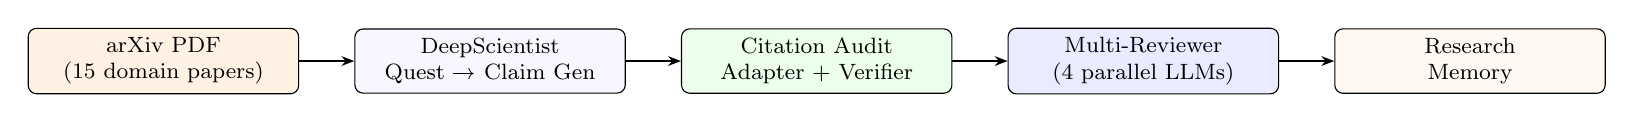
\begin{tikzpicture}[
  node distance=0.7cm,
  box/.style={rectangle, draw, rounded corners=3pt, fill=blue!3, text width=3.2cm, align=center, minimum height=0.8cm, font=\footnotesize},
  arrow/.style={-{Stealth[scale=0.7]}, thick},
]
  \node[box, fill=orange!10] (paper) {arXiv PDF\\(15 domain papers)};
  \node[box, right=of paper] (ds) {DeepScientist\\Quest → Claim Gen};
  \node[box, fill=green!8, right=of ds] (audit) {Citation Audit\\Adapter + Verifier};
  \node[box, fill=blue!8, right=of audit] (mr) {Multi-Reviewer\\(4 parallel LLMs)};
  \node[box, fill=orange!5, right=of mr] (mem) {Research\\Memory};

  \draw[arrow] (paper) -- (ds);
  \draw[arrow] (ds) -- (audit);
  \draw[arrow] (audit) -- (mr);
  \draw[arrow] (mr) -- (mem);
\end{tikzpicture}
\end{center}

\section{Agent 框架}

系统的代理层与验证层是分离的。代理层负责生成假设和引文主张，验证层负责逐条核查这些主张的真实性。这种分离使得两个阶段可以独立迭代：代理策略的调整不影响验证规则的稳定性，验证阈值的调优也不干扰代理的生成行为。

\textbf{代理循环}。系统提供两套生成路径。主路径（Path2）使用 DeepScientist 作为代理：DeepScientist 读取论文 PDF，通过其内置工具检索文献，生成结构化假设和引文，写入 claims JSON 文件。此过程中，DeepScientist 的 Claude 运行器自主管理工具调用和推理过程，系统仅通过 SKILL 文件约束输出格式和行为边界（例如禁止伪造 DOI、要求保守措辞）。

回退路径使用本地的 \texttt{CitationAuditClaimsGenerator}，它串联三个本地工具：PdfReaderTool（通过 pypdf 提取论文摘要和研究空白描述）、LiteratureSearcher（查询 Crossref、OpenAlex、Semantic Scholar、arXiv 获取相关文献），以及 HypothesisGenerator（基于论文摘要和检索结果生成假设 JSON）。这个本地管道在 DeepScientist 不可用或超时的情况下作为恢复路径。

\textbf{验证层}。验证层以 \texttt{CitationVerifier} 为核心，对其输入的每条 claim 执行四阶段检查：存在性查找（通过 DOI 或标题在四个公共 API 上查询）、版本消歧（当同一文献在多个数据源有不同记录时，按 DOI 精确匹配优先、标题-作者相似度次之的规则合并）、元数据比对（标题文本相似度、作者重叠度、发表年份匹配、DOI 精确匹配）、以及支撑度评分（将被引文献的摘要/片段与 claim 文本进行文本重叠和关键词覆盖分析）。综合打分后，每条 claim 被归入 Green（文献存在、元数据匹配、摘要直接支撑主张）、Yellow（文献存在但支撑不确定或部分匹配）或 Red（文献未找到、元数据不匹配或存在硬性矛盾）。

\textbf{LLM 的使用边界}。整个验证管道中，LLM 仅在两个环节被调用：HypothesisGenerator 中用于基于论文摘要和文献检索结果生成假设（这是创造性任务，需要 LLM），以及 CitationVerifier 中可选的单句解释生成（仅用于人工阅读，明确约束不得修改标签）。所有真值判断（引文是否存在、元数据是否正确、摘要是否支撑主张）均由确定性规则和公共 API 查询完成，不依赖 LLM 的判断。这一设计选择基于一个观察：LLM 在事实核验任务上存在确认偏误，倾向于将似是而非的引文标记为真实。

\section{Tool-Use 双层架构}

系统的工具调用采用双层设计：代理层使用 LLM 函数调用实现自主检索，验证层使用确定性 API 查询完成事实核验。两层之间通过工作流编排器衔接，工具调用的输入输出和耗时全部记录到审计日志中。

\subsection{代理层：LLM 驱动的函数调用}

HypothesisGenerator 是系统中唯一使用 LLM 函数调用的组件。它向 DeepSeek API 注册一个工具 \texttt{search\_literature}，定义为接受一组搜索查询字符串、返回学术论文元数据的函数。代理循环限制为最多三轮交互：

\begin{enumerate}[leftmargin=*,nosep]
  \item LLM 接收论文摘要和系统提示，自主决定是否调用 \texttt{search\_literature}。
  \item 若发出工具调用，工作流提取查询参数，通过 LiteratureSearcher 依次查询 Crossref、OpenAlex、Semantic Scholar 和 arXiv，合并去重后回传结果。
  \item 返回结果被裁剪为标题、作者和摘要前 500 字符，以 \texttt{role: "tool"} 消息格式匹配原始 \texttt{tool\_call\_id} 发回 LLM。
  \item LLM 评估检索结果，决定发起新搜索或输出最终假设 JSON。
\end{enumerate}

三轮结束后，agent 被强制要求输出符合预定义 schema 的结构化 JSON。该 schema 约束了每条假设必须包含的字段和每条引文必须具备的元数据项。

\begin{figure}[htbp]
\centering
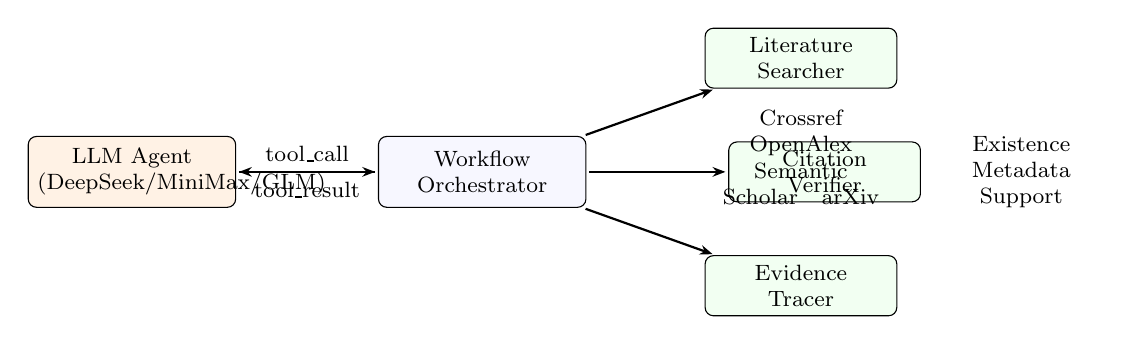
\begin{tikzpicture}[
  node distance=1.0cm and 1.8cm,
  box/.style={rectangle, draw, rounded corners=3pt, fill=blue!3, text width=2.4cm, align=center, minimum height=0.9cm, font=\footnotesize},
  apibox/.style={rectangle, draw, rounded corners=3pt, fill=green!5, text width=2.2cm, align=center, minimum height=0.7cm, font=\footnotesize},
  arrow/.style={-{Stealth[scale=0.7]}, thick, shorten >=1pt, shorten <=1pt},
]
  \node[box, fill=orange!10] (llm) {LLM Agent\\(DeepSeek/MiniMax/GLM)};
  \node[box, right=of llm] (wf) {Workflow\\Orchestrator};
  \node[apibox, above right=0.6cm and 1.5cm of wf] (lit) {Literature\\Searcher};
  \node[apibox, right=of wf] (cv) {Citation\\Verifier};
  \node[apibox, below right=0.6cm and 1.5cm of wf] (et) {Evidence\\Tracer};

  \draw[arrow] (llm) -- node[above, font=\footnotesize]{tool\_call} (wf);
  \draw[arrow] (wf) -- node[below, font=\footnotesize]{tool\_result} (llm);
  \draw[arrow] (wf) -- (lit);
  \draw[arrow] (wf) -- (cv);
  \draw[arrow] (wf) -- (et);

  \node[font=\footnotesize, below=0.15cm of lit, align=center, text width=2.4cm] {Crossref\quad OpenAlex\\Semantic Scholar\quad arXiv};
  \node[font=\footnotesize, right=0.15cm of cv, align=center, text width=2.0cm] {Existence\\Metadata\\Support};
\end{tikzpicture}
\caption{双层工具调用架构：左侧 LLM Agent 使用函数调用自主检索文献（最多 3 轮），右侧验证层以确定性 API 查询完成逐条引文核查。箭头方向表示数据流向，audit trail 全量记录。}
\label{fig:tool_arch}
\end{figure}

\subsection{验证层：确定性 API 查询}

CitationVerifier 不使用 LLM 函数调用。它的四个 API 查询函数各自封装了对一个公开数据源的 HTTP 请求：Crossref REST API、OpenAlex REST API、Semantic Scholar API、arXiv XML API。每个函数接收 DOI 或标题字符串，返回命中的候选文献元数据列表。查询策略是先按 DOI 精确查找（速度快、准确率高），若 DOI 为空或未命中则以标题搜索，结果集按引用数降序排列取前若干条。

验证管道按固定顺序执行：Lookup（依次调用四个 API）→ Version Resolution（同一文献的多源记录合并去重）→ Metadata Matching（标题相似度、作者 Jaccard 重叠、年份差、DOI 精确匹配综合打分）→ Support Scoring（abstract/snippet 句子级文本重叠与关键词覆盖率）→ Classification（九条件 Green Gate 判定）。Green Gate 的九个条件涵盖元数据匹配阈值、支撑分数下限、来源一致性、版本匹配状态等，全部满足方标记为 Green。LLM 仅用于 \texttt{\_llm\_explanation} 生成可读的审核说明，该函数的 docstring 明确声明其返回值不会导致标签升级。

\subsection{审计追踪}

系统中的每一次工具调用——无论是 LLM 驱动的 \texttt{search\_literature} 还是管道中的四个 API 查询——都通过 \texttt{ToolCallLogger} 写入运行目录下的 \texttt{tool\_calls.jsonl}。每条记录包含调用 ID、时间戳、工具名称、输入参数摘要、执行耗时、状态和错误信息。与之配合的 \texttt{EvidenceStore} 将每条工具调用产出的证据项（如查询到的文献记录、匹配到的候选条目）以证据 ID 关联回对应的工具调用，写入 \texttt{evidence\_items.jsonl}。两个日志文件共同构成从工具调用到证据项的完整审计链路。

\section{Research Memory 双层记忆}

系统包含两套独立的记忆机制，分别面向不同时间尺度和不同类别的幻觉风险。ResearchMemory 以文件持久化为基础，追踪跨运行引文可靠性；AgentMemory 以层级结构为框架，记录单代理的行为模式并自动归并为长期规则。

\subsection{ResearchMemory：跨运行引文审计记忆}

ResearchMemory 是一个基于 JSONL 的持久化存储，覆盖 \texttt{outputs/memory/} 下的五类文件：Citation Memory（按 DOI 或规范化标题键 upsert，累积每次运行中该引文的标签历史）、Provider Memory（记录各数据源在每次运行中的成功/失败计数）、Reviewer Memory（追加式记录每次多评审面板的评分和决策）、Failure Memory（按复合键 upsert，存储 Yellow/Red 级别的引文风险项）、以及 Case Memory（记录每个 case 每次运行的 Green/Yellow/Red 分布和最终评分）。

Upsert 操作的核心逻辑是：将目标 JSONL 文件全部加载到内存，按预定义的稳定键匹配；命中则合并新旧字段、递增 seen\_count、追加入 label\_history；未命中则初始化新条目、分配递增 memory\_id。写入采用整文件重写策略，该设计权衡了简单位操作的可读性和几百条记录规模的性能。

跨运行反幻觉的价值体现在三个机制上。其一，引文模式检测：当某 DOI 在历史运行中曾被标记为 Red，当前运行的 Multi-Reviewer 会收到该引文的完整标签历史作为评审上下文。其二，数据源可靠性追踪：跨运行累积的 API 错误计数使得审计者可以识别频繁返回错误的数据提供方。其三，标签历史融合：merge\_label\_history 确保一个运行中的 Green 标签不会覆盖该引文在历史上被判定为 Red 的事实，latest\_color\_label 始终反映最新运行结果，label\_history 保留完整演变记录。

\subsection{AgentMemory：层级化反思记忆}

AgentMemory 采用 Working / Short-term / Long-term 三层架构。Working Memory 是单次运行期间的计数器（已验证的 DOI 数、使用的数据源、各颜色标签计数）。Short-term Memory 记录近期的成功经验和验证错误，每条错误包含类型、详细原因和发生上下文。Long-term Memory 存储从 Short-term 中的重复模式自动压缩而来的规则，按 verification\_rules、provider\_insights 和 success\_patterns 三类分文件存储。

自动压缩的触发条件是：当 Short-term 中某 verification\_error 类型累积超过 30 条时，按 error\_type 分组、按 reason 去重后压缩为一条 Long-term verification\_rule。成功模式在 Short-term 中出现三次以上则晋升为 Long-term success\_pattern。压缩后的条目从 Short-term 中移除，保持 Short-term 的精简。

实际运行的反思数据中记录了三种高频错误类别：元数据伪造（LLM 编造了不存在的 DOI）、过度推断（在没有文本支撑的情况下做出跨领域论断）、以及引文幻觉（生成的 claim 与被引文献的实际内容矛盾）。这些反思以 Agent Reflection 块的形式注入 HypothesisGenerator 的系统提示中，使 agent 在生成新一轮假设时携带对过往错误的记忆。

\begin{figure}[htbp]
\centering
\begin{tikzpicture}[
  node distance=1.2cm,
  box/.style={rectangle, draw, rounded corners=3pt, fill=blue!3, text width=3.0cm, align=center, minimum height=0.9cm, font=\footnotesize},
  subbox/.style={rectangle, draw, rounded corners=3pt, fill=orange!5, text width=3.2cm, align=left, minimum height=0.85cm, font=\footnotesize},
  arrow/.style={-{Stealth[scale=0.7]}, thick},
]
  \node[box, fill=orange!12] (rm) {ResearchMemory\\跨运行 · 持久 · JSONL};
  \node[subbox, below=0.5cm of rm] (rmf) {citation record (upsert)\\| provider stats (upsert)\\| reviewer panel (append)\\| failure risks (upsert)\\| case summary (upsert)};

  \node[box, fill=blue!8, right=2.0cm of rm] (am) {AgentMemory\\单会话 · 层级 · 反思};
  \node[subbox, below=0.5cm of am] (amf) {Working: per-run counters\\| Short-term: recent errors\\| $\downarrow$ auto-compress (30+ / 3+)\\Long-term: rules \& patterns};

  \draw[arrow] (rm) -- (rmf);
  \draw[arrow] (am) -- (amf);

  \node[font=\footnotesize, above=0.05cm of rm, align=center] {目标：跨运行引文可靠性};
  \node[font=\footnotesize, above=0.05cm of am, align=center] {目标：单代理行为纠偏};
\end{tikzpicture}
\caption{双层记忆架构示意图。ResearchMemory 关注跨运行的引文级一致性，AgentMemory 关注单代理的行为级纠偏。两者独立运作，在 Multi-Reviewer 阶段汇合。}
\label{fig:memory_arch}
\end{figure}

\section{Multi-Reviewer 多模型平行评审}

Multi-Reviewer 是运行于引文验证之后的后审计面板。它对完整的假设包给出 1--6 的综合评分，产出 Accept / Revise / Reject 的三级决策。其核心设计约束是：确定性规则在评分上的优先级高于任何单一 LLM 的判断，LLM 不能通过高估计分覆盖由引文标签分布确定的硬性上限。

\subsection{架构：四模型平行评审}

不同于传统的角色分工（新颖性评审、证据评审、方法论评审、风险评审），当前设计将四位评审配置为完全平行的通用评审者。每位评审独立评估假设包的全部维度——新颖性、证据质量、方法论可检验性和潜在风险——而非各自聚焦于单一维度。四位评审使用四种不同的模型和三个不同的 API 提供商：

\begin{table}[htbp]
\centering
\caption{四位平行评审配置}
\begin{tabularx}{\textwidth}{@{}clll>{\raggedright\arraybackslash}X@{}}
\toprule
\textbf{ID} & \textbf{模型} & \textbf{提供商} & \textbf{API 端点} & \textbf{角色} \\
\midrule
R1 & deepseek-v4-flash  & DeepSeek & api.deepseek.com          & 通用评审（全维度） \\
R2 & deepseek-v4-pro    & DeepSeek & api.deepseek.com          & 通用评审（全维度） \\
R3 & minimax-text-01    & MiniMax  & api.minimax.chat          & 通用评审（全维度） \\
R4 & glm-4-flash        & GLM      & open.bigmodel.cn          & 通用评审（全维度） \\
\bottomrule
\end{tabularx}
\end{table}

这种设计的意图是：通过多模型、多提供商的独立评审获得对同一份审计结果的互补视角。不同模型的训练数据和偏好不同，其评分差异本身即为审计质量的一个信号。若四位评审在 Red 标签存在的条件下全部给出高分，这本身就是需要警惕的一致性偏差。评审之间不直接通信，不存在辩论或协调环节，每位的评分仅基于相同的审计上下文独立产生。

元评审（Meta-Reviewer）使用 DeepSeek V4 Pro，综合四份独立评审和确定性评分上限，产出加权后的最终分数和决策标签。

\begin{figure}[htbp]
\centering
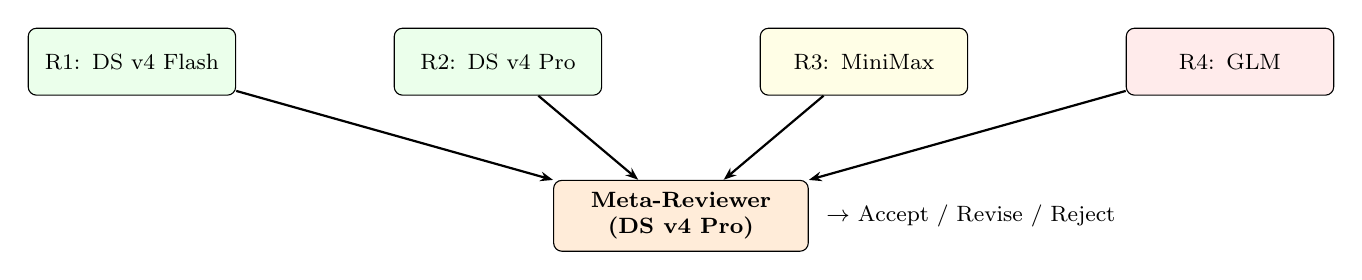
\begin{tikzpicture}[
  node distance=0.9cm and 2.0cm,
  reviewer/.style={rectangle, draw, rounded corners=3pt, fill=blue!5, text width=2.4cm, align=center, minimum height=0.85cm, font=\footnotesize},
  meta/.style={rectangle, draw, rounded corners=3pt, fill=orange!15, text width=3.0cm, align=center, minimum height=0.9cm, font=\footnotesize\bfseries},
  arrow/.style={-{Stealth[scale=0.7]}, thick},
]
  \node[reviewer, fill=green!8] (r1) {R1: DS v4 Flash};
  \node[reviewer, fill=green!8, right=of r1] (r2) {R2: DS v4 Pro};
  \node[reviewer, fill=yellow!10, right=of r2] (r3) {R3: MiniMax};
  \node[reviewer, fill=red!8, right=of r3] (r4) {R4: GLM};
  \node[meta, below=1.5cm of $(r2)!0.5!(r3)$] (meta) {Meta-Reviewer\\(DS v4 Pro)};

  \draw[arrow] (r1) -- (meta);
  \draw[arrow] (r2) -- (meta);
  \draw[arrow] (r3) -- (meta);
  \draw[arrow] (r4) -- (meta);

  \node[font=\footnotesize, right=0.1cm of meta, align=left] {$\rightarrow$ Accept / Revise / Reject};
\end{tikzpicture}
\caption{四模型平行评审架构。四位评审使用三种不同提供商的四种不同模型，独立对同一审计结果评分。元评审综合四份独立评审产出最终决策。}
\label{fig:multi_reviewer}
\end{figure}

\subsection{确定性评分上限}

\texttt{deterministic\_score\_cap} 是约束 LLM 评分不可逾越的硬上限，由引文标签的分布直接计算。初始值设为 6，逐级施加封顶规则：

\begin{table}[htbp]
\centering
\caption{评分上限触发规则}
\begin{tabularx}{\textwidth}{@{}>{\ttfamily}l>{\raggedright\arraybackslash}Xc@{}}
\toprule
\textbf{触发条件} & \textbf{规则} & \textbf{Cap} \\
\midrule
any\_red\_claim          & 存在任意 Red 标签引文                                  & 2 \\
red\_line\_error\_type   & 检测到硬性引文错误（not\_found、doi\_metadata\_mismatch 等） & 2 \\
yellow\_majority         & Yellow 占比超过 50\%                                   & 3 \\
no\_green\_claims        & 没有引文通过九条件 Green Gate                            & 3 \\
support\_risk\_error     & 主张过强 / 关键词缺失 / 数值矛盾                          & 3 \\
risk\_penalty\_total     & 确定性风险罚分累计 $\ge 3$                                & 4 \\
\bottomrule
\end{tabularx}
\end{table}

取最低上限为有效 Cap。Cap 为 2 时强制 Reject；Cap 为 3 时最多允许 Revise，禁止 Accept。每位评审的 LLM 输出分数在 normalize 阶段被夹紧至不超过该 Cap，元评审的最终分数同样受此约束。

\subsection{双模式运行与降级策略}

系统支持三种运行模式：auto（检测到 API 密钥则用 LLM，否则降级为确定性规则）、deepseek（强制使用 LLM，但密钥缺失时仍降级）、deterministic（完全跳过 LLM，仅用规则评分）。确定性模式下的评分逻辑基于引文标签的形状计算：以 Green 数量为基础分、Yellow 占比和 Red 数量为扣分项、Green Gate 通过率为上限。该模式确保了即使所有外部 API 均不可用，系统仍能产出有依据的评审结果。

\subsection{评审一致性与冲突消解}

四位评审分数的一致程度由极差度量：极差不大于 1 为高一致性，不大于 2 为中一致性，超过 2 为低一致性。元评审在合成最终决策时会考虑一致性水平，但冲突的根本解决机制是确定性评分上限。极端情况下，即使四位 LLM 评审全部给出满分 6 分，若引文标签中存在 Red 记录，Cap 机制将最终分数强制截断为 2，决策强制为 Reject。

\section{实现概要}

整个系统由以下核心模块构成：

\begin{table}[htbp]
\centering
\caption{核心源文件}
\begin{tabularx}{\textwidth}{@{}l>{\raggedright\arraybackslash}X@{}}
\toprule
\textbf{模块} & \textbf{职责} \\
\midrule
\texttt{agent/deepscientist\_adapter.py} & DeepScientist 适配主入口：标准化、富化、验证编排 \\
\texttt{agent/deepscientist\_claims\_normalizer.py} & 将 DS 多格式输出规范化为验证器输入 schema \\
\texttt{agent/hypothesis\_generator.py} & 定义 search\_literature 工具，实现 3 轮代理循环 \\
\texttt{agent/citation\_verifier.py} & 确定性引文验证：4 个公共 API 查询 + 5 阶段判定管道 \\
\texttt{agent/research\_memory.py} & 跨运行 JSONL 持久记忆：5 类记录，upsert/append/lookup \\
\texttt{agent/agent\_memory.py} & 三层反思记忆：Working → Short-term → Long-term 自动压缩 \\
\texttt{agent/workflow.py} & 本地工作流编排（回退路径） \\
\texttt{agent/run\_logging.py} & 审计日志：ToolCallLogger + EvidenceStore \\
\texttt{agent/llm\_client.py} & LLM 客户端工厂：DeepSeek / MiniMax / GLM 统一调用接口 \\
\texttt{scripts/run\_multi\_reviewer.py} & 多评审面板：4 位平行评审 + 元评审，含 Cap 机制 \\
\texttt{scripts/run\_official\_ds\_case.py} & 单案例 Path2 管道：Quest → DS Run → Audit → Review → Memory \\
\texttt{scripts/deepscientist\_15x\_campaign.py} & 15 案例泛化压力测试批处理 \\
\bottomrule
\end{tabularx}
\end{table}

系统通过统一的 \texttt{call\_llm} 接口支持 DeepSeek、MiniMax 和 GLM 三个 LLM 后端，通过 httpx 配置跳过代理和信任环境变量以确保内网环境下的请求稳定性。所有对外部 API 的调用均设置超时，异常路径通过 Python 异常机制统一走确定性降级逻辑。

\end{document}
